\documentclass[a4paper, openany, 14pt]{article}

%% подключаем стандарт библиографии
\bibliographystyle{gost71u}

%% для "Abstract" в классе book
% \newenvironment{abstract}{}{}
% \usepackage{abstract}

%% подключаем преамбулу: в ней содержится подключение всех необходимых пакетов
%% Работа с русским языком
\usepackage{cmap}			 % поиск в PDF
\usepackage{mathtext} 		 % русские буквы в формулах
\usepackage[T2A]{fontenc}	 % кодировка
\usepackage[utf8]{inputenc}	 % кодировка исходного текста
\usepackage[russian]{babel}	 % локализация и переносы

%% Пакеты для работы с математикой
\usepackage{amsmath,amsfonts,amssymb,amsthm,mathtools}
\usepackage{icomma}
\usepackage{etoolbox}

%% Нумерация формул (опционально)
%\mathtoolsset{showonlyrefs=true} % показывать номера только у тех формул, на которые есть \eqref{} в тексте.
%\usepackage{leqno}               % нумерация формул слева

%% Шрифты
\usepackage{euscript}	 % шрифт "Евклид"
\usepackage{mathrsfs}    % красивый мат. шрифт

%% Некоторые полезные макросы для дебага (в случае недоверия авторам шаблона)
\makeatletter
\newcommand\thefontsize{The current font size is: \f@size pt} % пример: \section{\thefontsize}
\makeatother

%% Настройка размеров шрифтов
\makeatletter
\setlength{\headheight}{28pt}
%% TODO: мне не удалось разобраться, как грамотно подбирать второе число в 
%% \@setfontsize\*, но ряд эксппериментов показывает, что "10" выравнивает текст весьма прилично :)
\renewcommand\Huge{\@setfontsize\Huge{14pt}{10}}
\renewcommand\huge{\@setfontsize\huge{14pt}{10}}
\renewcommand\Large{\@setfontsize\Large{14pt}{10}}
\renewcommand\large{\@setfontsize\large{12pt}{10}}
\makeatother

%% Поля (геометрия страницы)
\usepackage[left=3cm,right=1.5cm,top=2cm,bottom=2cm,bindingoffset=0cm]{geometry}

%% Русские списки
\usepackage{enumitem}
\makeatletter
\AddEnumerateCounter{\asbuk}{\russian@alph}{щ}
\makeatother

%% Работа с картинками
\usepackage{caption}
\captionsetup{justification=centering} % центрирование подписей к картинкам
\usepackage{graphicx}                  % вставки рисунков
\graphicspath{{images/}{images2/}}     % папки с картинками
\setlength\fboxsep{3pt}                % отступ рамки \fbox{} от рисунка
\setlength\fboxrule{1pt}               % толщина линий рамки \fbox{}
\usepackage{wrapfig}                   % обтекание рисунков и таблиц текстом

%% Работа с таблицами
\usepackage{array,tabularx,tabulary,booktabs} % дополнительная работа с таблицами
\usepackage{longtable}                        % длинные таблицы
\usepackage{multirow}                         % слияние строк в таблице

%% Красная строка
\setlength{\parindent}{2em}

%% Интервалы
\linespread{1.5}
\usepackage{multirow}

%% TikZ
\usepackage{tikz}
\usetikzlibrary{graphs,graphs.standard}

%% Верхний колонтитул
\usepackage{fancyhdr}
\pagestyle{fancy}

%% Перенос знаков в формулах (по Львовскому)
\newcommand*{\hm}[1]{#1\nobreak\discretionary{}{\hbox{$\mathsurround=0pt #1$}}{}}

%% Дополнительно
\usepackage{float}   % добавляет возможность работы с командой [H] которая улучшает расположение на странице
\usepackage{abstract}
\usepackage{gensymb} % красивые градусы
\usepackage{caption} % пакет для подписей к рисункам, в частности, для работы caption*
\usepackage{listings} % пакет для листингов с кодом
\lstset{              % настройки для лисингов с кодом
basicstyle=\small\ttfamily,
columns=flexible,
breaklines=true
}

% Hyperref (для ссылок внутри  pdf)
\usepackage[unicode, pdftex]{hyperref}

% Отступ перед первым абзацем в каждом разделе
\usepackage{indentfirst}


\begin{document}
    %% титульник
    \begin{center}
    %% *название института*
    \large\textbf{Министерство образования и науки Российской Федерации \\
    Московский физико-технический институт (государственный
    университет)} \\
    \vspace{1cm}

    %% *факультет/физтех-школа*
    Физтех-школа радиотехники и компьютерных технологий \\

    %% *название базовой кафедры и лаборатории*
    %% в случае ненадобности можно удалить
    Кафедра микропроцессорных технологий в интеллектуальных системах
 управления \\

    \vspace{3em}

    Выпускная квалификационная работа бакалавра
\end{center}

\begin{center}
    \vspace{\fill}
    %% *название вашей работы*
    \LARGE{Название будет сгенерировано на сервисе МФТИ}

    \vspace{\fill}
\end{center}


\begin{flushright}
    \textbf{Автор:} \\
    Вчера это был я \\
\end{flushright}

\vspace{7em}

\begin{center}
    %% *лого*
    
\includegraphics[width=100 pt]{MIPT_logo.jpg}\\
    Москва \the\year{}
\end{center}

%% выключаем отображение номера для этой страницы (титульник)
\thispagestyle{empty}

\newpage
\setcounter{page}{2}
\fancyfoot[c]{\thepage}
%% *надпись над верхним колонтинулом*
%% в случае ненадобности можно удалить
\fancyhead[L]{Исследование методов визуализации неевклидовых пространств}
\fancyhead[R]{}
    \fontsize{14}{16}\selectfont
    %% аннотоция
    \renewcommand{\abstractnamefont}{\normalfont\Large\bfseries}
\renewcommand{\abstracttextfont}{\normalfont\Huge}

\begin{center}
    \textbf{Аннотация}
\end{center}

В данной работе исследуются методы визуализации неевклидовых пространств в режиме реального времени с целью сравнения их производительности, а также качества получаемых изображений при их использовании. Рассмотрены такие методы визуализации, как марширование и трассировка лучей, а также метод предварительного расчета. Методы визуализации реализованы посредством графического API \textit{Vulkan} \cite{vulkan}. Основным результатом работы является усовершенствованный метод рендеринга сложных сцен в пространственно-временном поле с сильным искривлением со сторонней геометрией.
\vfill

\newpage
    %% содержание
    \tableofcontents{}
    \newpage

    \section{Введение}
\label{sec:Chapter0} \index{Chapter0}

Компьютерная графика с самого своего создания использовала для описания расположения объектов в пространстве набор \textit{(x, y, z, w)} координат, называемых \textit{однородными}. Их удобно использовать при описании евклидова пространства, поскольку первые три компоненты представляют из себя декартовы координаты. Эти координаты легко преобразовывать матрицами преобразования, такими как матрицы масштабирования, переноса и поворота.

Неевклидово пространство же не всегда можно описать такими однородными координатами. Более того, возможны пространства в которых нельзя ввести систему координат в принципе. Таким пространством, например, является пространство общей теории относительности, в котором происходит искривление.

Актуальность работы обусловлена потребностью визуализации черных дыр, червоточин и прочих искривленных пространств при реализации научных идей, в частности касающихся общей теории относительности. Не менее востребована необходимость визуализации неевклидовых пространств в видеоигровой индустрии, что подтверждается серией игр \textit{Portal}.

Выбор черной дыры в качестве неевклидова пространства в данной работе обусловлен следующими факторами:
\begin{itemize}
  \item Актуальностью применения исследуемых методов визуализации в научных целях.
  \item Возможностью реализации метода рендеринга (визуализации) неевклидовых пространств со сторонней геометрией.
  \item Возможностью реализации альтернативного метода рендеринга, оптимизирующего производительность.
\end{itemize}

Таким образом, в качестве рабочей сцены, на основании которой будут реализовываться различные методы рендеринга, выбрана черная дыра.

\textbf{\textit{Целью}} настоящей работы является исследование и реализация методов рендеринга неевклидовых пространств в режиме реального времени на примере искривленного черной дырой пространства. При этом при определенной доработке предлагаемых методов прогнозируется возможность их использования для более сложных случаев, таких как двойная статическая черная дыра или даже червоточина.

Для достижения указанной цели поставлены следующие \textbf{\textit{задачи}}:

\begin{enumerate}
  \item Реализовать алгоритм рендеринга черной дыры.
  \item Реализовать альтернативный алгоритм рендеринга черной дыры, оптимизирующий производительность.
  \item Реализовать  усовершенствованный алгоритм рендеринга черной дыры, позволяющий отрисовывать стороннюю геометрию.
  \item Сравнить производительность реализованных методов рендеринга.
\end{enumerate}

\newpage
 %% Введение
    \section{Алгоритм рендеринга черной дыры}
\label{sec:Chapter1} \index{Chapter1}

Рендеринг реалистичного изображения в компьютерной графике можно сравнивать с фотосъемкой. И там, и там конечным результатом является изображение, которое получается на основании свойств света, попавшего в камеру. Пользуясь этим, можно упростить законы выбранного неевклидова пространства, используя их только для света (фотонов).

\subsection{Метрика Шварцшильда}

В науке наиболее популярным методом описания пространства является метрика - симметричное тензорное поле ранга (0,2) на гладком многообразии, посредством которого задаётся скалярное произведение векторов в касательном пространстве. Иначе говоря, благодаря метрике можно понять как при малых изменениях локальных (т.е. применимых только в локальной области) координат $(dx, dy, ...)$ изменяется расстояние $ds$ между точками в пространстве. Примеры метрик:
\begin{itemize}
  \item Евклидова: $ds^2=dx^2+dy^2+dz^2$.
  \item Сферическая (двумерная): $ds^2=dx^2+cos^2(\frac{y}{R})dy^2$.
  \item Минковского: $ds^2=c^2dt^2-dx^2-dy^2-dz^2$.
\end{itemize}

Для описания выбранной рабочей сцены, т.е. для черной дыры (предполагая, что она не заряжена и не вращается), существует метрика Шварцшильда в сферических координатах $(t, r, \theta, \phi)$:
\begin{equation}
\label{eq:schwarzschild_metric}
    ds^2 = c^2d\tau^2 = (1-\frac{r_s}{r})c^{2}dt^{2} - (1-\frac{r_s}{r})^{-1}dr^2 - r^2(d\theta^2+sin^2(\theta)d\phi^2)
\end{equation}
, где $\tau$ - собственное время и $r_s = \frac{2GM}{c^2}$ - \textit{радиус Шварцшильда}, который определяет область вокруг ЧД массой $M$, которую луч света покинуть не сможет. Считаем, что центр черной дыры расположен в начале координат.

Для частиц в течение движения сохраняются энергия и угловой момент (константы движения):
\begin{equation}
\label{eq:motion_constant_E}
    E = (1-\frac{r_s}{r})\frac{dt}{d\tau}.
\end{equation}

\begin{equation}
\label{eq:motion_constant_L}
    L = r^2\frac{d\phi}{d\tau}.
\end{equation}

Метрику можно преобразовать из \eqref{eq:schwarzschild_metric}, считая $c = 1$ и $\theta=\frac{\pi}{2}$, поскольку метрика Шварцшильда симметрична, а значит траектория луча всегда будет лежать в плоскости:
\begin{equation}
\label{eq:schwarzschild_metric1}
    c^2 = (1-\frac{r_s}{r})c^2(\frac{dt}{d\tau})^2 - (1-\frac{r_s}{r})^{-1}(\frac{dr}{d\tau})^2 - r^2(\frac{d\phi}{d\tau})^2.
\end{equation}

Из \eqref{eq:motion_constant_E}, \eqref{eq:motion_constant_L} и \eqref{eq:schwarzschild_metric1} можно получить следующее выражение:
\begin{equation}
\label{eq:schwarzschild_metric2}
    (\frac{dr}{d\tau})^2 = \frac{E^2}{m^2c^2} - (1-\frac{r_s}{r})(c^2+\frac{L^2}{r^2}).
\end{equation}

Поскольку справедливо следующее равенство:
\begin{equation}
\label{eq:equation_of_diff}
    (\frac{dr}{d\phi})^2 = (\frac{dr}{d\tau})^2(\frac{d\tau}{d\phi})^2 = (\frac{dr}{d\tau})^2(\frac{r^2}{L})^2.
\end{equation}

То используя \eqref{eq:schwarzschild_metric2} и \eqref{eq:equation_of_diff} можно получить уравнение:
\begin{equation}
\label{eq:schwarzschild_metric3}
    (\frac{dr}{d\phi})^2 = \frac{r^4}{b^2} - (1-\frac{r_s}{r})(\frac{r^4}{a^2} + r^2).
\end{equation}
, где $a = \frac{L}{c}$ и $b = \frac{mcL}{E}$ - константы.

Применяя замену переменной $u = \frac{1}{r}$, а также учитывая, что при стремлении массы частицы $m$ к нулю, $m \longrightarrow 0$, константа движения $a$ стремиться к бесконечности, $a \longrightarrow \infty$, упрощаем \eqref{eq:schwarzschild_metric3}:
\begin{equation}
\label{eq:schwarzschild_metric4}
    (\frac{du}{d\phi})^2 = r_su^3 - u^2 + \frac{1}{b^2}.
\end{equation}

Дифференцируя \eqref{eq:schwarzschild_metric4}:
\begin{equation}
\label{eq:schwarzschild_metric5}
    2\frac{du}{d\phi}\frac{d^2u}{d\phi^2} = 3r_su^2\frac{du}{d\phi} - 2u\frac{du}{d\phi}.
\end{equation}

Итоговый результат из \eqref{eq:schwarzschild_metric5} выглядит следующим образом:
\begin{equation}
\label{eq:diffur}
    \frac{d^2u}{d\phi^2} = \frac{3}{2}r_su^2 - u.
\end{equation}

\subsection{Методы Рунге-Кутты}
\label{subsec:runge-kutte}

Дифференциальное уравнение \eqref{eq:diffur} не имеет явного решения, поэтому разумно использовать для его решения итеративный подход. Одними из таких подходов являются методы Рунге-Кутты.

Методы Рунге-Кутты позволяют итеративно находить решение дифференциальных уравнений с заданными условиями на сетке $\phi$ значений, обычно с постоянным шагом $\Delta \phi$:

\begin{equation}
\label{eq:runge-kutte}
    \frac{\mathbf{dy}}{d\phi} = \mathbf{f}(\phi, \mathbf{y}),
    \quad
    \left.\mathbf{y}\right|_{\phi=\phi_0}=\mathbf{y_0}.
\end{equation}

В случае уравнения \eqref{eq:diffur}:

\begin{equation*}
\label{eq:runge-kutte_y}
    \mathbf{y} =
    \begin{cases}
        u
        \\
        \frac{du}{d\phi}
    \end{cases}
\end{equation*}

\begin{equation*}
\label{eq:runge-kutte_f}
    \mathbf{f}(\phi, \mathbf{y}), =
    \begin{cases}
        \frac{du}{d\phi}
        \\
        \frac{3}{2}r_su^2 - u
    \end{cases}
\end{equation*}

Для данной работы были выбраны явные методы Рунге-Кутты порядков 1, 2 и 4. Разные порядки имеют разную точность, сведения представлены в таблице \ref{tab:runge-kutte}:

\begin{center}
    \begin{table}[h!]
        \centering
        \begin{tabular}{|c|c|}
            \hline
            Порядок метода Рунге-Кутты & Погрешность шага $\Delta h$ \\
            \hline
            Рунге-Кутты 1-го порядка (RK1) & $O(h^2)$ \\
            \hline
            Рунге-Кутты 2-го порядка (RK2) & $O(h^3)$ \\
            \hline
            Рунге-Кутты 4-го порядка (RK4) & $O(h^5)$ \\
            \hline
        \end{tabular}
        \caption{Сравнение погрешностей методов Рунге-Кутты.}
        \label{tab:runge-kutte}
    \end{table}
\end{center}


\subsection{Инициализация лучей света}
\label{subsec:ray_init}

Осталось только определить $y_0$ и $\phi_0$ из \eqref{eq:runge-kutte}. Начальные условия $y_0$ будут определяться на основе позиции и направления камеры (т.е. наблюдателя), а также угла обзора (field of view).

\begin{figure}[h]
    \centering
    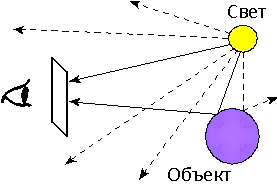
\includegraphics[width=0.5\linewidth]{CameraRaysProblem}
    \caption{Малая часть испущенного света попадает в камеру.}
    \label{fig:camera_rays_problem}
\end{figure}

Стоит отметить, что, как было сказано выше, рендеринг - это свет попавший в камеру. Но испускать свет в сцене от всех источников освещения, а затем учитывать только тот свет, что попал в камеру - невыгодно, поскольку лишь малая часть действительно попадет в камеру (см. рис. \ref{fig:camera_rays_problem}). Поэтому в компьютерной графике давно используют закон обратимости света: гораздо выгоднее выпускать лучи из каждого пикселя камеры и затем просчитывать какой цвет они приобретут в ходе движения по сцене.

\begin{figure}[h]
    \centering
    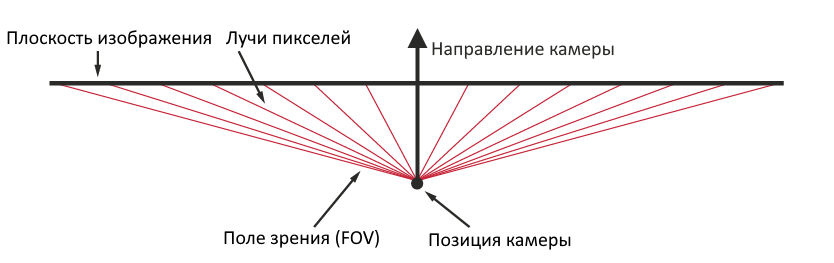
\includegraphics[width=1.0\linewidth]{PinholeCameraModel}
    \caption{Модель камеры-обскуры (pinhole camera model).}
    \label{fig:pinhole_camera}
\end{figure}

В качестве модели камеры выбрана модель камеры-обскуры \\(pinhole camera model) \cite[стр.~47]{marrs2021ray}, поскольку это одна из стандартных моделей камеры. Для ее настройки необходимо знать параметры камеры и угол обзора (поле зрения). Главным следствием использования этой модели является эквидистантность точек пересечения лучей с плоскостью изображения, лежащих на одной линии (см. рис. \ref{fig:pinhole_camera}).

Пусть изображение представляет из себя тензор второго ранга размером $(N, M)$. Индекс пикселя это упорядоченный набор двух неотрицательных чисел $(n, m)$, начиная с $0$ по каждому пикселю. Направление и позиция в декартовых координатах, а также угол обзора камеры обозначаются $\mathbf{a_c}$, $\mathbf{d_c}$ и $fov$ соответственно. В терминологии данной работы углом обзора будет называться угол между крайними лучами на одной горизонтальной прямой. Зная все это можно получить направления лучей каждого пикселя в декартовых координатах $\mathbf{d_0}$:

\begin{align*}
    x &= (n + 0.5)/N, \\
    y &= (m + 0.5)/M, \\
    scale_{horizontal} = scale_h &= \tan{\left(\frac{fov}{2}\right)}, \\
    scale_{vertical} = scale_v &= \left(\frac{N}{M}\right) \cdot scale_h, \\
    \mathbf{offset}_{horizontal} = \mathbf{offset}_h &= scale_h \cdot normalize(\mathbf{d_c} \times \mathbf{e_z}), \\
    \mathbf{offset}_{vertical} = \mathbf{offset}_v &= scale_v \cdot normalize(\mathbf{d_c} \times \mathbf{offset}_h).
\end{align*}

Таким образом, направление луча пикселя в декартовых кооринатах $\mathbf{d_0}$ можно вычислить следующим образом:

\begin{equation}
\label{eq:init_rays}
    \mathbf{d_{nm}} = \mathbf{d_c} + \mathbf{offset}_{h} \cdot x + \mathbf{offset}_{v} \cdot y.
\end{equation}

\subsection{Переход из декартовых в полярные координаты плоскости вращения}

Полученные начальные условия $\mathbf{d_0}$ из \eqref{eq:init_rays} получены в декартовых координатах, а метод Рунге-Кутты, изложенный в разделе \ref{subsec:runge-kutte}, описан в полярных координатах. Поэтому перед итеративным решением необходимо определить $y_0$ и $\phi_0$ из \eqref{eq:runge-kutte} на основании данных раздела \ref{subsec:ray_init}.

\newpage

\begin{figure}[h]
    \centering
    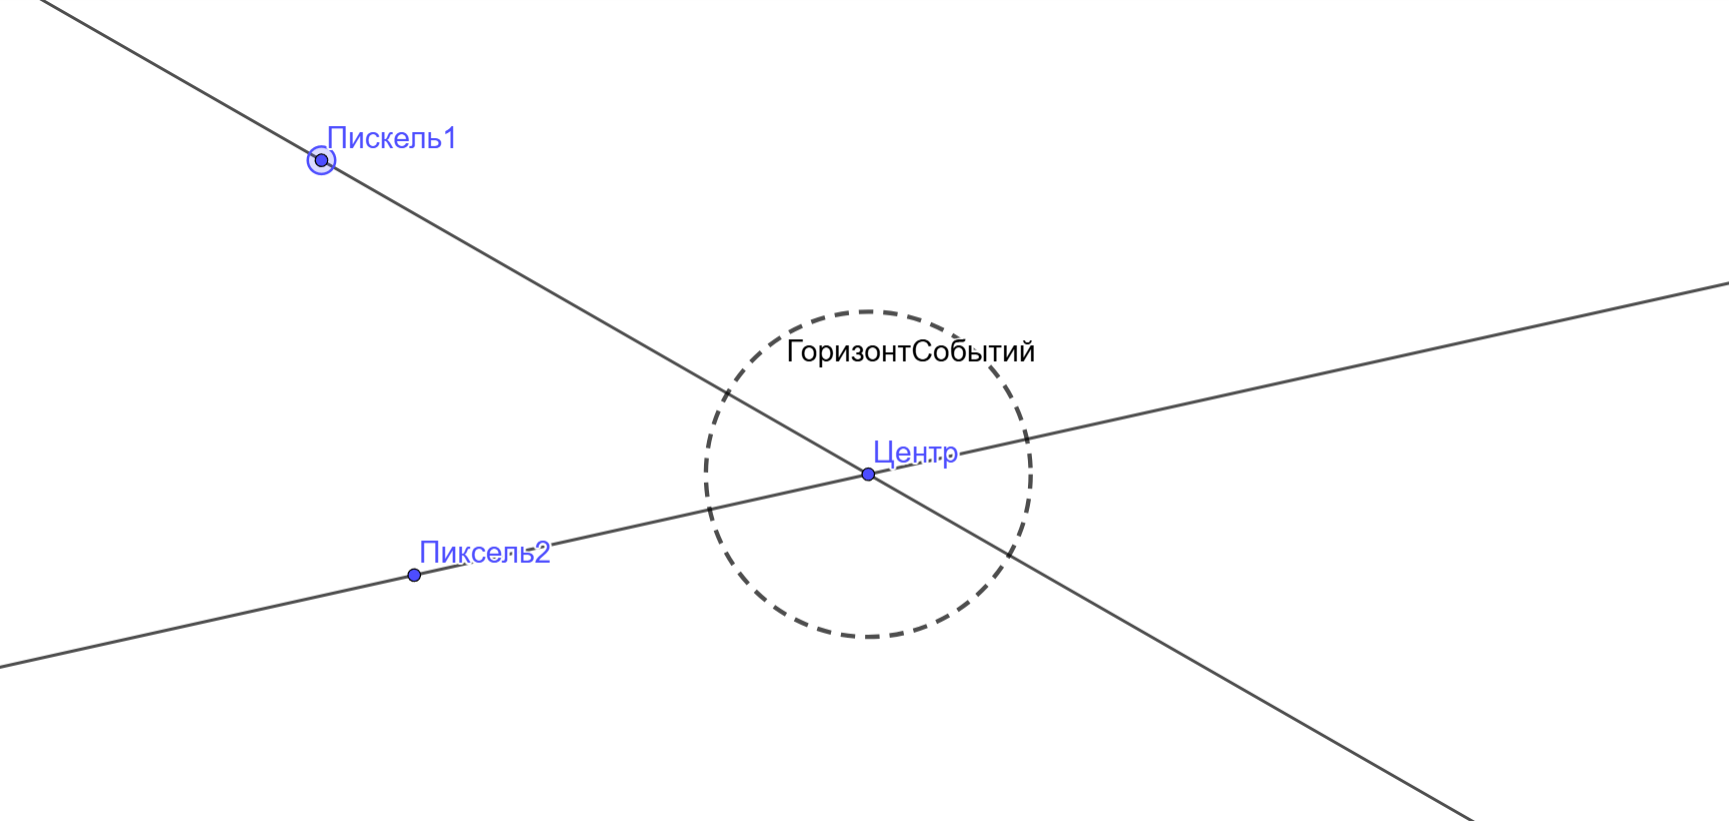
\includegraphics[width=1.0\linewidth]{rotation_plane}
    \caption{Разные плоскости вращения с точки зрения камеры.}
    \label{fig:rotation_plane}
\end{figure}

Для простоты примем $\phi_0 = 0$. Начальный радиус $r_0 = |\mathbf{a_c}|$, т.е. начальный обратный радиус $u_0 = \frac{1}{r_0} = \frac{1}{|\mathbf{a_c}|}$. Таким образом первая компонента $\mathbf{y_0}$ определена.

Для нахождения второй компоненты сперва нужно определить вектор вращения луча $\mathbf{w_{nm}}$ т.е. вектор, задающий плоскость вращения. В общем случае для каждого пикселя плоскость вращения будет отличаться (см. рис. \ref{fig:rotation_plane}).

\begin{equation}
\label{eq:w_ray}
    \mathbf{w_{nm}} = \mathbf{a_c} \times \mathbf{d_{nm}}.
\end{equation}

\newpage

\begin{figure}[h]
    \centering
    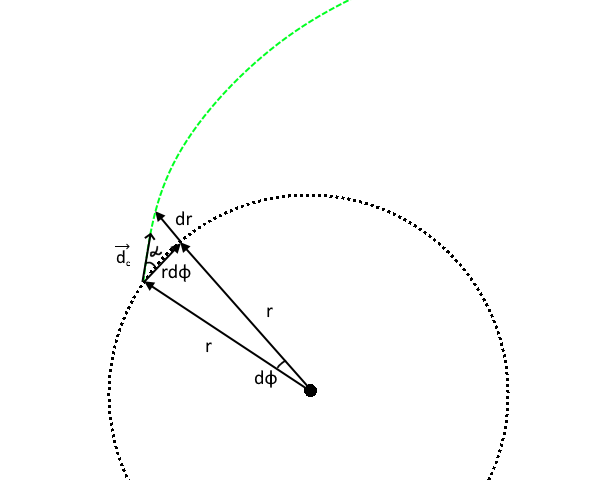
\includegraphics[width=0.8\linewidth]{BlackHole-RayAngle}
    \caption{Начальные условия (зеленым изображена траектория света, черным пунктиром - окружность, центр которой совпадает с центром черной дыры).}
    \label{fig:blackhole_rayAngle}
\end{figure}

Поскольку вторая компонента $\mathbf{y_0}$ это $\frac{du}{d\phi}$, то необходимо вычислить начальное значение этой производной (см. рис. \ref{fig:blackhole_rayAngle}), пользуясь методом малых перемещений:

\begin{equation}
\label{eq:dudr_init}
    \left.\frac{du}{d\phi}\right|_{\phi=\phi_0=0} = \frac{d\left(\frac{1}{r}\right)}{d\phi} = -\frac{1}{r^2}\left(\frac{dr}{d\phi}\right) = -\frac{\tan{\alpha}}{r} = -\frac{1}{r}\left(\frac{\mathbf{a_c} \cdot \mathbf{d_{nm}}}{\left|\mathbf{w_{nm}}\right|}\right).
\end{equation}

Подытоживая, начальное условие $\mathbf{y_0}$ будет равно:

\begin{equation}
\label{eq:runge-kutte_y0}
    \mathbf{y_0} =
    \begin{cases}
        \frac{1}{\left|\mathbf{a_c}\right|}
        \\
        -\frac{1}{r}\left(\frac{\mathbf{a_c} \cdot \mathbf{d_{nm}}}{\left|\mathbf{w_{nm}}\right|}\right)
    \end{cases}
\end{equation}

\newpage

\subsection{Краевые случаи}
\label{subsec:corner_cases}
Для черной дыры выделяются два краевых случая:

\begin{enumerate}
    \item Попадание луча в горизонт событий.
    \item Уход луча на бесконечность.
\end{enumerate}

Рассмотрим каждые из них отдельно.

\subsubsection{Попадание луча в горизонт событий}
\label{subsubsec:events_horizon}

Луч, попавший в горизонт событий, уже никогда не выйдет из него, поэтому можно сказать, пользуясь законом обратимости света, что такие лучи приобретают черный цвет (если по пути до этого не пересеклись с другим объектом, разумеется).

Поскольку \textit{радиус Шварцшильда} $r_s$ является радиусом горизонта событий, то на каждой итерации решения уравнения \eqref{eq:diffur} методом Рунге-Кутты необходимо проводить проверку на нахождение внутри шара горизонта событий. То есть если на $i$-ой итерации, $r_i = \frac{1}{u_i} < r_s$, то нужно остановить итерирование и обрабатывать полученный результаты.

\subsubsection{Уход луча на бесконечность}
\label{subsubsec:goes_to_infinity}

Луч, находящийся далеко от черной дыры, движется по почти прямой траектории. В таком случае можно считать, что направление луча не измениться, а значит можно сразу окрасить луч света в какой-то цвет на основании \textit{дальнего} окружения черной дыры.

\newpage

\begin{figure}[h]
    \centering
    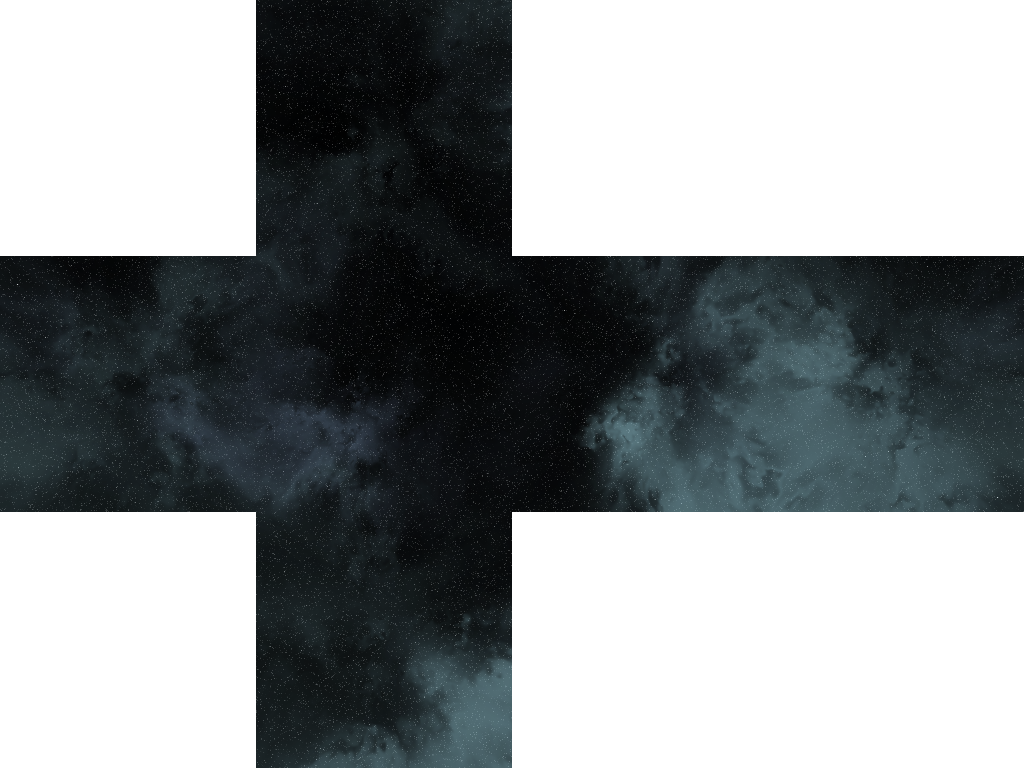
\includegraphics[width=1.0\linewidth]{cubemap}
    \caption{Кубическая текстура звездного неба.}
    \label{fig:cubemap}
\end{figure}

Черные дыры - это массивные объекты, находящиеся в космосе. Поэтому в качестве окружения разумно выбрать звездное небо (см. рис. \ref{fig:cubemap}) и в случае ухода луча на бесконечность брать значения из этого звездного неба.

Осталось определить условие ухода луча на бесконечность. В общем случае на каждой $i$-ой итерации стоило бы проверять, как далеко свет ушел, но для черной дыры можно сделать упрощение, которое несет в себе еще и решение различных визуальных проблем: когда луч уходит все дальше и дальше от черной дыры, то $\phi$ из \eqref{eq:diffur} почти перестает меняться, что может вызывать проблемы с постоянным шагом $\Delta\phi$ в методе Рунге-Кутты. Упрощенное условие ухода на бесконечность выглядит следующим образом (см. рис. \ref{fig:blackhole_rayAngle}):

\begin{equation}
\label{eq:goes_to_infinity}
    \tan{\alpha} > tan_{crit} \quad \textit{или} \quad \left(\frac{du}{d\phi}\right)_i < -tan_{crit} \cdot u.
\end{equation}
, где $tan_{crit}$ - критическое значение тангенса угла $\alpha$ к окружности с центром, совпадающим с центром черной дыры.

\subsection{Аккреционный диск}
\label{subsec:accr_disk}

Все прошлые разделы описывали реализацию \textit{гравитационного линзирования}. Однако стоит отметить, что по соседству с черной дырой часто оказывается вращающийся горячий газовый диск, именуемый \textit{аккреционным диском}. Аккреционный диск по своим размерам сопоставим с радиусом Шварцшильда во всех направлениях (в том числе и в толщине) и поскольку это горячий газ, то его можно воспринимать как полупрозрачный объект.

Сложность визуализации аккреционного диска зависит от желаемого уровня реалистичности. Для данной работы я ограничился следующими параметрами аккреционного диска: ось вращения диска, внутренний и внешний радиусы, а также сделал цвет диска зависящим только от радиуса и расстояния от плоскости, задаваемой осью вращения диска.

\newpage
 %% Алгоритм рендеринга черной дыры
    \section{Предрасчитанные данные}
\label{sec:Chapter2} \index{Chapter2}

Помимо очевидных оптимизаций, например изменения шага итерирования или уменьшения разрешения итогового изображения, для некоторых сцен возможны оптимизации, координально меняющие алгоритм рендеринга. Для рабочей сцены, т.е. для черный дыры, возможно одна из таких оптимизаций - можно использовать заранее расчитанные данные, чтобы не использовать метод Рунге-Кутты \eqref{eq:runge-kutte} множество раз в цикле, а просто взять необходимую информацию из этих предрасчитанных данных. Для черной дыры этими данными будут информация об итоговом угле отклонения $\phi$ луча на бесконечности для корректной отрисовки окружающей среды и информация о пересечении луча с аккреционного диска.

\subsection{Итоговый угол отклонения $\phi$ на бесконечности}
\label{subsec:precomputed_phi}

Начальный угол в разделе \ref{subsec:transition_from_decart_to_polar} приняли за ноль $\phi_{0} = 0$. Для итогового угла отклонения $\phi$ нельзя получить аналитическое выражение, однако можно заранее рассчитать итоговый угол $\phi$ при уходе луча на бесконечность и записать ее в качестве \textit{текстуры} (изображения), из которой затем будет выбираться необходимая информация. Текстуру удобно использовать, поскольку для текстур предлагается аппаратная линейная фильтрация на видеокарте между пикселями текстуры.

Итак, для рассчета итогового угла отклонения необходимо знать значения параметров $u$ и $\frac{du}{d\phi}$ из уравнения \eqref{eq:diffur}. Действительно, поскольку траектория света в окрестности черной дыры не зависит от вектора вращения, т.е. вектора плоскости, в которой луч совершает движение, то можно ограничиться только этими двумя параметрами. Таким образом, поскольку необходимо знать два параметра, то предрасчитанная текстура будет двумерной. Разумеется каждый пиксель будет хранить данные типа \textit{float32} (IEEE-754).

Рассчитать значения можно тем же методом Рунге-Кутты, но поскольку это предрассчет, то можно использовать более точные порядки и шаги итерирования.

В ходе итерирования луч также может попасть в горизонт событий и такой случай нужно как-то записать. В данной работе помимо итогового значения угла отклонения $\phi$ записывается еще маска, идентифицирующая попадание в черную дыру: если луч попал в черную дыру, то записывается значение $-1.0$, если луч ушел на бесконечность - записывается $1.0$. Таким образом каждому пикселю текстуры соответсвует набор из двух значений $\left(\phi, \text{mask}\right)$.

Осталось разобраться что будет означать ось абсцисс текстуры, а что будет означать ось ординат. Самое главное требование - компактность координат. Координаты должны пробегать все возможные значения, но при этом являться ограниченными. Примером неподходящего параметра является радиус $r$. Луч в алгоритме рендеринга черной дыры (см. раздел \ref{sec:Chapter1}) принимает следующие значения радиуса $r \in \left[r_{s}, +\infty\right]$ и этот параметр не подходит, поскольку может уйти на бесконечность. С другой стороны, параметр $u=\frac{1}{r} \in \left[0, \frac{1}{r_s}\right]$ вполне подходящий, т.к. область значений находится на конечном промежутке. Поэтому для оси абсцисс был выбран нормализованный обратный радиус:

\begin{equation}
\label{eq:sample_precompute_u}
    \frac{r_s}{r}=ur_s \in [0, 1].
\end{equation}

, a для оси ординат - угол:

\begin{equation}
\label{eq:sample_precompute_alpha}
    \left(\frac{\alpha}{\pi} + 0.5\right) \in \left[0, 1\right].
\end{equation}

, угол $\phi$ аналогичен углу с тем же названием из раздела \ref{subsec:transition_from_polar_to_decart} (см. рис. \ref{fig:transform_direction}). Напомню, что $\frac{du}{d\phi} = -\frac{1}{r} \cdot \tan{\phi}$.

Резюмируя, предрассчет будет выглядеть следующим образом: для каждого пикселя текстуры размером $(X, Y)$ с координатами $(x_i, y_i)$ будут линейно вычисляться обратный радиус и угол $phi$ по формулам, обратным формулам \eqref{eq:sample_precompute_u} и \eqref{eq:sample_precompute_alpha}:

\begin{equation}
\label{eq:precompute_u}
    u = \frac{1}{r} = \frac{1}{r_s} \cdot \frac{x_i}{X - 1}.
\end{equation}

\begin{equation}
\label{eq:precompute_alpha}
    \alpha = \pi\cdot\left(\frac{y_i}{Y - 1} - 0.5\right),
    \quad
    \frac{du}{d\phi} = -\frac{1}{r}\tan{\alpha}.
\end{equation}

, а зная $u$ и $\frac{du}{d\phi}$ уже по известному алгоритму можно рассчитать итоговый угол отклонения $\phi$ (см. рис. \ref{fig:precomputed_phi}).

\begin{figure}[h]
    \centering
    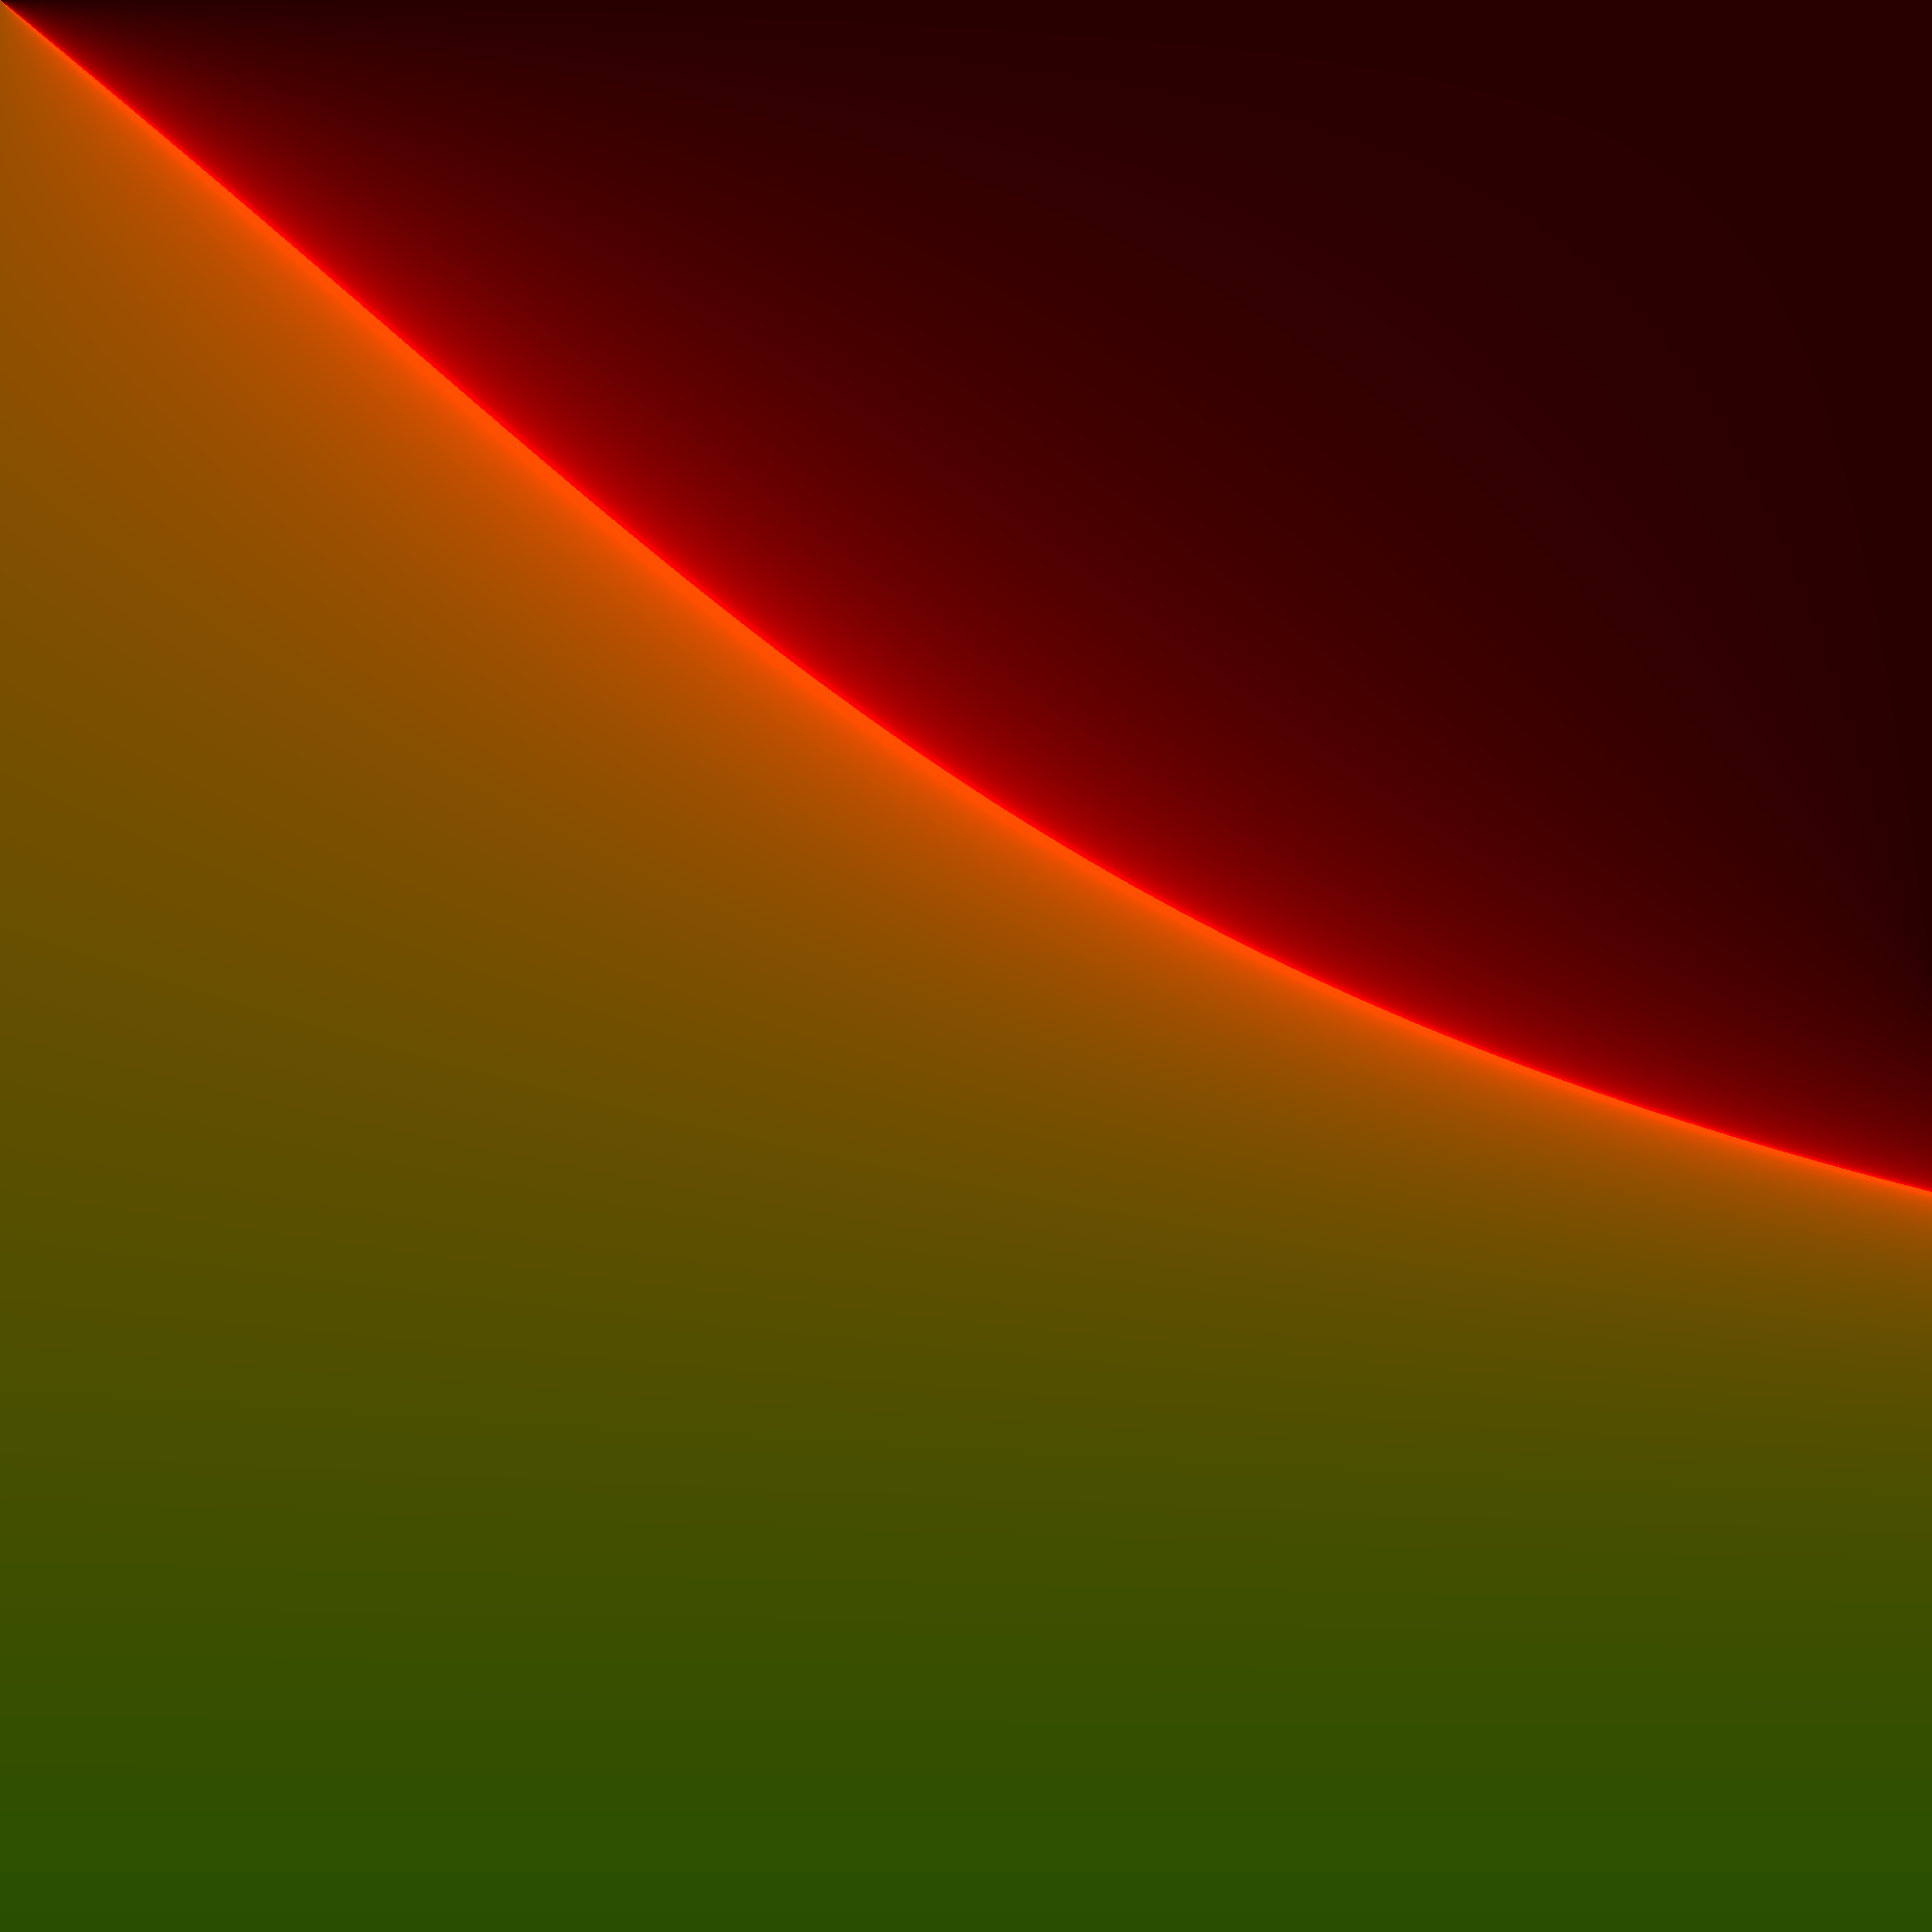
\includegraphics[width=0.8\linewidth]{PrecomputedPhi}
    \caption{Предрасчитанная текстура размером $(2000, 2000)$. Красный канал отвечает за итоговый угол отклонения $\phi$, а зеленый канал - за маску, идентефицирующую попадание в горизонт событий.}
    \label{fig:precomputed_phi}
\end{figure}

\newpage

\subsection{Пересечение луча с аккреционным диском}

\begin{figure}[h]
    \centering
    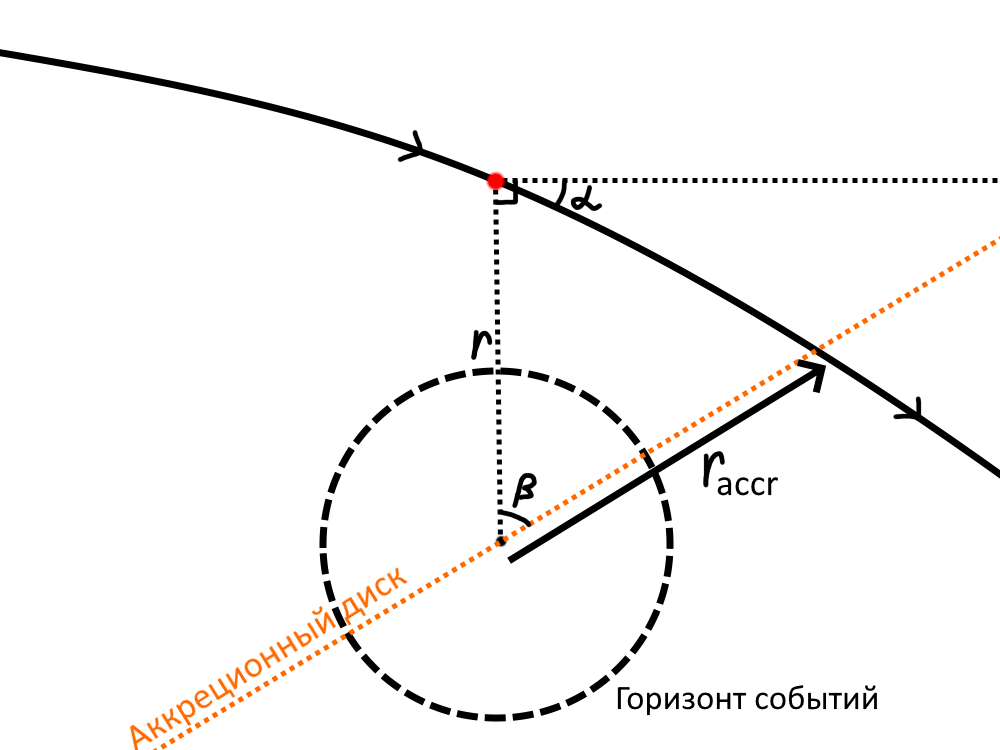
\includegraphics[width=0.8\linewidth]{Angles-Overview}
    \caption{Схема параметров для предрассчета радиуса пересечения $r_{accr}$ аккреционного диска. Сплошной кривой указана траектория света вблизи черной дыры, оранжевым пунктиром - линия пересечения плоскости аккреционного диска и плоскости движения луча света.}
    \label{fig:angle_overview}
\end{figure}

В случае аккреционного диска, зависимость плотности которого радиальна, согласно разделу \ref{subsec:accr_disk}, достаточно лишь знать радиус пересечения с аккреционным диском $r_{accr}$, при условии, что диск является очень тонким.

Для того, чтобы узнать радиус пересечения с аккреционным диском $r_{accr}$ нужно дополнительно знать угол $\beta$ до пересечения с аккреционными диском в плоскости движения луча света, помимо параметров $u$ и $\alpha$ из прошлого раздела \ref{subsec:precomputed_phi} (см. рис. \ref{fig:angle_overview}). Поскольку необходимо знать три параметра для нахождения искомого $r_{accr}$, то текстура будет трехмерной размером $(X, Y, Z)$.

Ось абсцисс и ось ординат текстуры такие же, как в прошлом разделе \ref{subsec:precomputed_phi}. А вот ось аппликат будет с координатами равными:

\begin{equation}
\label{eq:sample_precompute_beta}
    \frac{\beta}{\pi} \in \left[0, 1\right].
\end{equation}

Таким образом, алгоритм вычисления радиуса пересечения с аккреционным диском $r_{accr}$ следующий: для каждого пикселя в предрассчитанной текстуре с координатами $(x_i, y_i, z_i)$ вычисляются $u$ и $\alpha$ по формулам \eqref{eq:precompute_u} и \eqref{eq:precompute_alpha}, а параметр $\beta$ вычисляется по формуле, обратной \eqref{eq:sample_precompute_beta}:

\begin{equation}
\label{eq:precompute_beta}
    \beta = \pi \cdot \frac{z_i}{Z - 1}.
\end{equation}

Зная $u$, $\frac{du}{d\phi}$ и $\beta$ легко вычислить искомое значение $r_{accr}$. Для этого используем все тот же метод Рунге-Кутты, однако заменяем всего пару вещей: начальное значение $\phi=\phi_0$ делаем равным $\beta$ и добавляем условие на пересечение с аккреционным диском, а именно при достижении параметра $\phi$ значения $\pi$ или больше, считаем пересечения луча света с аккреционным диском произошедшим и записываем радиус $r = \frac{1}{u}$ в пиксель. Если луч ушел на бесконечность, то нужно записать какой-то идентифицирующее это значение, например большое число. Если же луч попал в горизонт событий, то нужно использовать еще одно специальное значение, например ноль.

Обычно при наблюдении черной дыры хорошо видно два аккреционных диска, возникающих при первом и втором пересечениях траектории света с аккреционным диском, поэтому разумно в текстуре сохранять набор из двух значений: радиусы первого и второго пересечений с аккреционным диском $r_{accr1}$ и $r_{accr2}$.

Рисунки \ref{fig:precomputed_accr_beta_1pi4} и \ref{fig:precomputed_accr_beta_3pi4} показывают предрасчитанные радиусы $r_{accr}$ для первого и второго пересечений с аккреционным диском для значений $\beta = \frac{1\pi}{4}$ и $\beta = \frac{3\pi}{4}$ соответственно. Наблюдаются три зоны: черная - либо траектория света ушла в горизонт событий, не успев пересечься с аккреционным диском, либо первый пересечение произошло, а второе - нет, либо первое и второе пересечения с аккреционным диском произошли; зеленая - траектория света пересекла плоскость аккреционного диска лишь один раз; желтая - траектория света не пересекла ни разу плоскость аккреционного диска.

\newpage

\begin{figure}
    \centering
    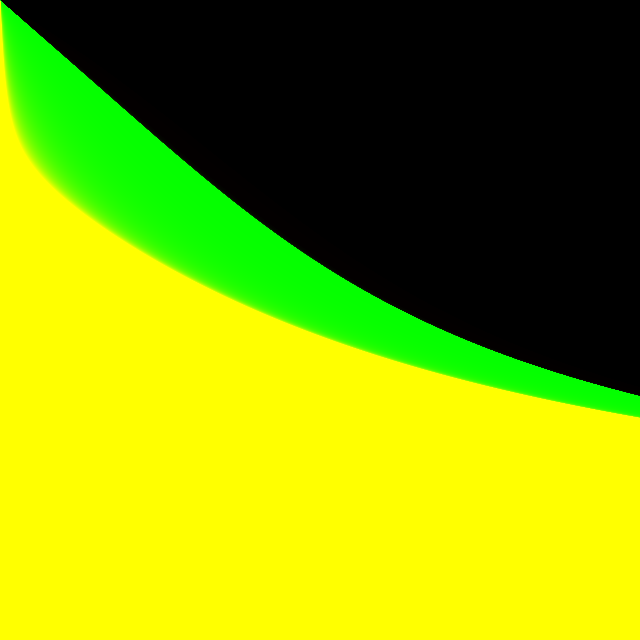
\includegraphics[width=0.45\linewidth]{PrecomputedAccrBetapi4}
    \caption{Предрасчитанная текстура размером $(640, 640, 128)$, но выбрано значение $\beta = \frac{\pi}{4}$. Красный канал отвечает за радиус первого пересечения с аккреционным диском $r_{accr1}$, а зеленый канал - за радиус первого пересечения с аккреционным диском $r_{accr2}$.}
    \label{fig:precomputed_accr_beta_1pi4}
\end{figure}

\begin{figure}[h]
    \centering
    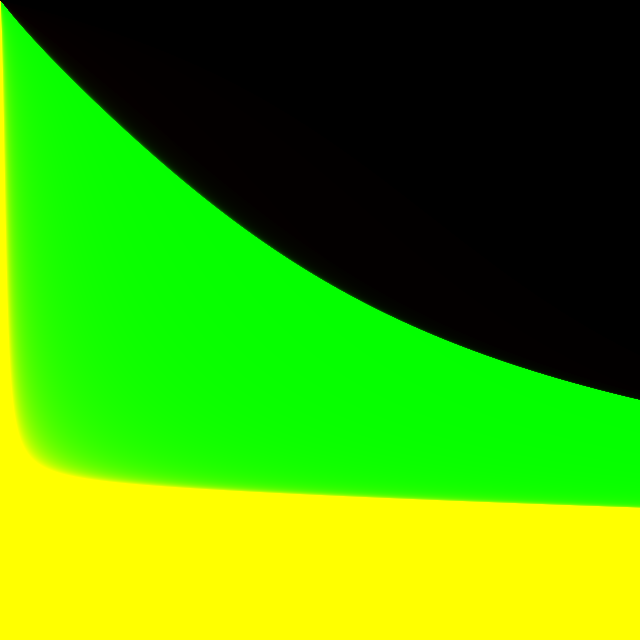
\includegraphics[width=0.45\linewidth]{PrecomputedAccrBeta3pi4}
    \caption{Предрасчитанная текстура размером $(640, 640, 128)$, но выбрано значение $\beta = \frac{3\pi}{4}$. Красный канал отвечает за радиус первого пересечения с аккреционным диском $r_{accr1}$, а зеленый канал - за радиус первого пересечения с аккреционным диском $r_{accr2}$.}
    \label{fig:precomputed_accr_beta_3pi4}
\end{figure}

\newpage

\subsection{Использование предрасчитанных данных для рендеринга черной дыры}
\label{subsec:precompute_black_hole_rendering}

Как было сказано выше, теперь для рендеринга черной дыры необходимо только использовать предрасчитанные данные и затем обработать их.

Для аккреционного диска, выбирая данные по координатам \eqref{eq:sample_precompute_u}, \eqref{eq:sample_precompute_alpha} и \eqref{eq:sample_precompute_beta}, можно получить данные о радиусе пересечений с аккреционным диском, а зная их, можно легко определить цвет в месте пересечения (как я и говорил выше, цвет диска имеет исключительно радиальную зависимость в данной работе).

Для итогового угла отклонения $\phi$ можно рассчитать как измениться позиция луча света $\mathbf{a}$ на бесконечности, а поскольку это происходит на бесконечности, то в пределе можно сказать, что позиция $\mathbf{a}$ и направление $\mathbf{d}$ луча света будут сонаправлены, а значит легко можно будет взять цвет из окружающей среды (см. раздел \ref{subsubsec:goes_to_infinity}).

Единственным минусом предрасчитанных данных является допущение малой толщины аккреционного диска.

\begin{figure}[h]
    \centering
    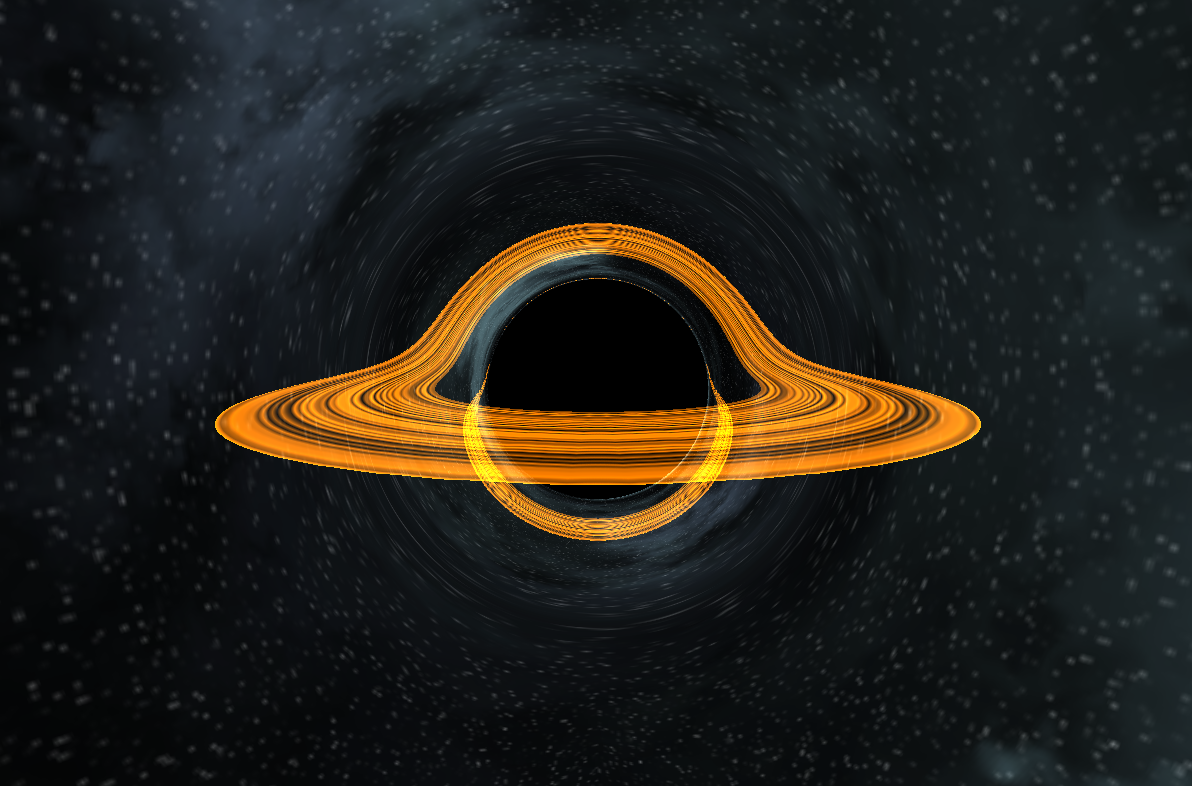
\includegraphics[width=1.0\linewidth]{BlackHolePrecomputed}
    \caption{Рендеринг черной дыры с использованием предрасчитанных данных.}
    \label{fig:black_hole_precomputed}
\end{figure}

\newpage %% Предрасчитанные данные
    \section{Общий метод рендеринга неевклидовых пространств}
\label{sec:Chapter3} \index{Chapter3}

Под общим методом рендеринга подразумевается добавление любого объекта в неевклидово пространство с его правильной визуализацией, в соответствии с законами неевклидова пространства.

Эта глава будет посвящена добавлению объектов на рабочую сцену с черной дырой.

\subsection{Триангулированные объекты}
\subsection{Обновленный алгоритм рендеринга черной дыры}

\newpage %% Общий метод рендеринга неевклидовых пространств
    % !TeX encoding = UTF-8
% !TeX spellcheck = ru_RU

\section{Результаты}
\label{sec:Chapter4} \index{Chapter4}

\subsection{Характеристики устройства для тестов}

Перед обсуждением результатов, стоит привести характеристики устройства, использованного для тестирования реализованных методов:

\begin{itemize}
    \item CPU: 12th Gen Intel(R) Core(TM) i7-12650H
    \item Встроенное GPU: Intel(R) UHD Graphics
    \item Дискретное GPU: NVIDIA GeForce RTX 4070 Laptop GPU
    \item ОЗУ: 16GB
\end{itemize}
, где GPU - это графический процессор или видеокарта, а CPU - центральный процессор.

\subsection{Графическое API Vulkan}

Для рендеринга было выбрано графическое API \textit{Vulkan}, поскольку он является кроссплатформенным графическим API нового поколения (к новым относят \textit{DirectX 12}, \textit{Metal} и \textit{Vulkan}, к старым - \textit{OpenGL}, \textit{DirectX 11} и ниже), предоставляет более обширное управление для работы с видеокартой и обладает возможностью использования новых технологий последних лет (например сеточный шейдер (mesh shader) и трассировка лучей (ray tracing)).

\begin{figure}[h]
    \centering
    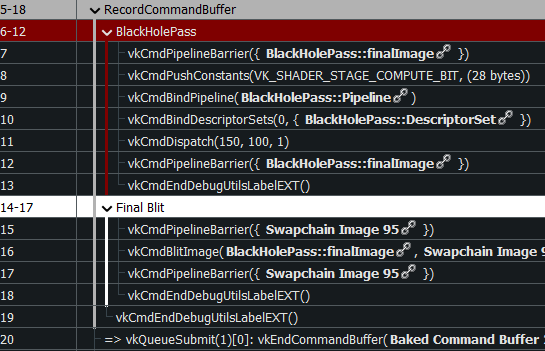
\includegraphics[width=0.8\linewidth]{CommandBuffer}
    \caption{Список команд, исполняющихся на GPU на каждом кадре. Получено при помощи приложения \textit{RenderDoc}.}
\end{figure}

Для всех методов используется \textit{Vulkan 1.0}, если не заявлено иначе. Все команды, исполняющиеся на GPU можно поделить на две группы:

\begin{enumerate}
    \item Визуализация черной дыры в вычислительном шейдере.
    \item Копирование вычисленного изображения в цепочку изображений \linebreak(swapchain) для последующего отображения на дисплей.
    \label{item:blit}
\end{enumerate}
, где вычислительный шейдер - аналог CUDA и OpenCL программ, исполняемых на GPU. Шаг \ref{item:blit} является крайне легковесным и почти не влияющим на производительность.

\begin{figure}[h]
    \centering
    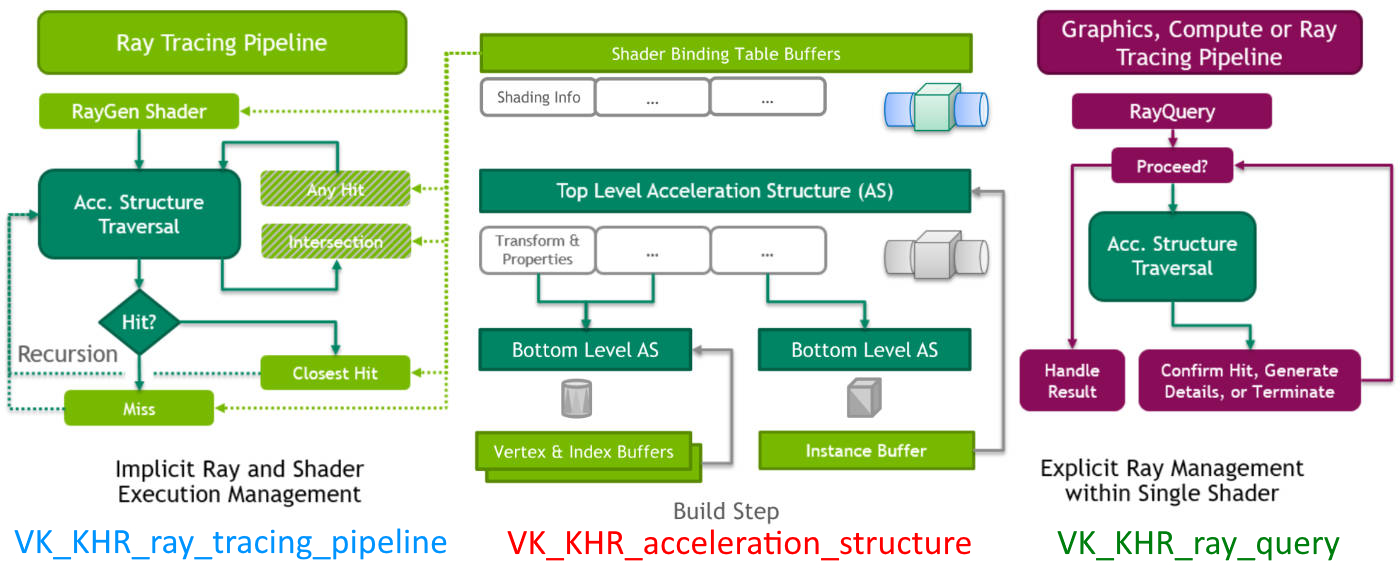
\includegraphics[width=1.0\linewidth]{Ray-Tracing-Overview}
    \caption{Набор расширений \textit{Vulkan Ray Tracing}.}
    \label{fig:raytracing_overview}
\end{figure}

При использовании трассировки лучей используется \textit{Vulkan 1.2} с набором расширений \textit{Ray Tracing} (см. рис. \ref{fig:raytracing_overview}): ускоряющие структуры\linebreak (acceleration structures), конвейер трассировки лучей (ray tracing pipeline) и запрос лучей (ray query). В работе используются первое и последнее расширения.

Ускоряющие структуры (acceleration structures) предоставляют скрытую реализацию иерархии ограничивающих объемов (bounding volume\linebreak hierarchy), чтобы совершать быстрый обход всей геометрии на сцене для поиска пересечения с лучем.

Запрос луча (ray query) нужен для самой трассировки лучей. Это расширение является альтернативой расширению конвейера трассировки лучей (ray tracing pipeline), но выделяет ее легкость использования, меньшая нагрузка на драйвер GPU, а также возможность использования в различных, в том числе фрагментных и \underline{вычислительных} шейдерах, что крайне полезно в случае данной работы.

\subsection{Сравнение реализованных методов}

\subsubsection{Визуальная составляющая}

Визуальный результат представлен на рисунках \ref{fig:black_hole_ray_marching}, \ref{fig:black_hole_precomputed} и \ref{fig:blackhole_raytracing}, а также в Приложении Б.

Если использовать реализацию марширования лучей (см. раздел \ref{sec:Chapter1}) для сравнения с другими, то в случае предвычисленных данных (см. раздел \ref{sec:Chapter2}) аккреционный диск превратился из трехмерного в двумерный объект, а в случае реализации комбинации марширования лучей и трассировки лучей - добавление новых объектов.

\subsubsection{Производительность}

Производительность будет измеряться в количестве \textbf{вычисленных}, а не отображенных на дисплее, кадров в секунду (frames per second, FPS). Разница существенная - количество отображенных кадров ограничено частотой обновления дисплея, а количество вычисленных кадров ограничено только мощностью устройства. Тем самым будет измеряться реальная производительность методов. В API \textit{Vulkan} это делается указанием \verb|VK_PRESENT_MODE_MAILBOX_KHR| при выборе режима представления цепочки изображений (swapchain).

Итак, результаты представлены ниже:

\begin{center}
    \begin{table}[h!]
        \centering
        \begin{tabular}{|c|cccccc|}
        \hline
        \multirow{3}{*}{GPU} & \multicolumn{6}{c|}{FPS}                                                                                                                                                                                                                      \\ \cline{2-7} 
                             & \multicolumn{2}{c|}{RK1}                                                             & \multicolumn{2}{c|}{RK2}                                                             & \multicolumn{2}{c|}{RK4}                                        \\ \cline{2-7} 
                             & \multicolumn{1}{c|}{$\Delta\phi = 0.003$} & \multicolumn{1}{c|}{$\Delta\phi = 0.01$} & \multicolumn{1}{c|}{$\Delta\phi = 0.003$} & \multicolumn{1}{c|}{$\Delta\phi = 0.01$} & \multicolumn{1}{c|}{$\Delta\phi = 0.003$} & $\Delta\phi = 0.01$ \\ \hline
        RTX 4070 Laptop      & \multicolumn{1}{c|}{190}                  & \multicolumn{1}{c|}{630}                 & \multicolumn{1}{c|}{175}                  & \multicolumn{1}{c|}{588}                 & \multicolumn{1}{c|}{141}                  & 470                 \\ \hline
        Intel UHD Graphics   & \multicolumn{1}{c|}{33}                   & \multicolumn{1}{c|}{100}                 & \multicolumn{1}{c|}{25}                   & \multicolumn{1}{c|}{79}                  & \multicolumn{1}{c|}{17}                   & 53                  \\ \hline
        \end{tabular}
        \caption{Производительность метода рендеринга черной дыры маршированием лучей (раздел \ref{subsec:algos}).}
        \label{tab:results_raymarching}
    \end{table}
\end{center}

Отчетливо видно падение производительности при увеличении порядка метода Рунге-Кутты, поскольку с увеличением порядка увеличивается и вычислительная сложность алгоритма. Также с уменьшением шага метода Рунге-Кутты $\Delta\phi$ также увеличивается производительность в связи с уменьшением количества итераций. Дополнительно следует отметить падение производительности при переходе с RTX 4070 Laptop на Intel UHD Graphics.

\begin{center}
    \begin{table}[h!]
        \centering
        \begin{tabular}{|c|c|}
        \hline
        GPU                & FPS  \\ \hline
        RTX 4070 Laptop    & 9950 \\ \hline
        Intel UHD Graphics & 330  \\ \hline
        \end{tabular}
        \caption{Производительность метода рендеринга черной дыры при помощи предрасчитанных данных (раздел \ref{subsec:precompute_black_hole_rendering}).}
        \label{tab:results_precomputed}
    \end{table}
\end{center}

Наблюдается прирост FPS в десятки раз в случае использования предрасчитанных данных по сравнению с маршированием лучей. Однако за такой прирост необходимо платить большим использованием видеопямяти для хранения предрасчитанных данных (например в данной работе для трехмерной текстуры предрассчитанных данных аккреционного диска размером $(640, 640, 128)$ и содержащем в каждом своем пикселе по два значения типа \textit{float32} (IEEE-754) занятый объем видеопамяти составляет примерно 400 мегабайт).

\begin{center}
    \begin{table}[h!]
        \centering
        \begin{tabular}{|c|cc|}
        \hline
        \multirow{3}{*}{GPU} & \multicolumn{2}{c|}{FPS}                                        \\ \cline{2-3} 
                             & \multicolumn{2}{c|}{RK1}                                        \\ \cline{2-3} 
                             & \multicolumn{1}{c|}{$\Delta\phi = 0.003$} & $\Delta\phi = 0.01$ \\ \hline
        RTX 4070 Laptop      & \multicolumn{1}{c|}{18}                   & 60                  \\ \hline
        \end{tabular}
        \caption{Производительность метода рендеринга черной дыры комбинацией марширования лучей и трассировки лучей (раздел \ref{subsec:new_algos}).}
        \label{tab:results_raymarchingtracing}
    \end{table}
\end{center}

Использование трассировки лучей очень сильно влияет на производительность, поскольку она используется на каждой итерации. Поэтому наблюдается падение производительности по сравнению с обычным маршированием лучей в примерно десять раз.

\newpage %% Обсуждение результатов

    %% НЕ ТРОГАЙТЕ!!!
    \nocite{*}
    \bibliography{references}

    %% в зависимости от надобности подключаем раздел "Приложение"
    % \newpage
    % \section*{Приложение}
\addcontentsline{toc}{section}{Приложение}
\label{sec:Apendix} \index{Apendix}

Здесь необходимо написать приложение, которое вы должны придумать самостоятельно.

\end{document}
